\documentclass%
%[handout]
{beamer}
% % % % % % % %
% % % % % % % %
% % % % % % % %
%IMPORTANT
%compiles with 
%pdflatex -shell-escape 
%IMPORTANT
% % % % % % % %
% % % % % % % %
% % % % % % % %
\mode<presentation>
{
\useinnertheme{rounded}
\useoutertheme{infolines}
\usecolortheme{orchid}
\usecolortheme{whale}
}

\usepackage[english]{babel}
\usepackage[latin1]{inputenc}
\usepackage[all,cmtip]{xy}
\usepackage{times}
\usepackage[T1]{fontenc}
\usepackage{../example-templates}
\usepackage{../pstricks-commands}

\usepackage{auto-pst-pdf}
\usepackage{pst-plot}
%\usepackage{pstricks-add} 

% Or whatever. Note that the encoding and the font should match. If T1
% does not look nice, try deleting the line with the fontenc.

\graphicspath{{../../modules/}}

\newtheoremstyle{partialproof}{3pt}{3pt}{}{}{}{.}{.5em}{}
\theoremstyle{partialproof} \newtheorem{partialproof}[theorem]{Proof.}
%\DeclareMathOperator{\diff}{d}
\newcommand{\diff}{\text{d}}
\setbeamertemplate{navigation symbols}{}

\includeonlylecture{1}

\newcommand{\lect}[3]{
  \date{#1}
  \lecture[#1]{#2}{#3}
}

\setbeamertemplate{footline}
{
  \leavevmode%
  \hbox{%
  \begin{beamercolorbox}[wd=.333333\paperwidth,ht=2.25ex,dp=1ex,center]{author in head/foot}%
    \usebeamerfont{author in head/foot}\insertshortauthor
  \end{beamercolorbox}%
  \begin{beamercolorbox}[wd=.333333\paperwidth,ht=2.25ex,dp=1ex,center]{title in head/foot}%
    \usebeamerfont{title in head/foot}\insertshorttitle
  \end{beamercolorbox}%
  \begin{beamercolorbox}[wd=.333333\paperwidth,ht=2.25ex,dp=1ex,center]{date in head/foot}%
    \usebeamerfont{date in head/foot}\insertshortdate{}
  \end{beamercolorbox}}%
  \vskip0pt%
}

% If you have a file called "university-logo-filename.xxx", where xxx
% is a graphic format that can be processed by latex or pdflatex,
% resp., then you can add a logo as follows:

%\pgfdeclareimage[height=0.8cm]{logo}{bluelogo}
%\logo{\pgfuseimage{logo}}

\begin{document}

\AtBeginLecture{%

\title[\insertlecture]{FreeCalc}
\subtitle{\insertlecture}
\author[FreeCalc]{}
\institute[UMass Boston]{University of Massachusetts Boston}
\date{\insertshortlecture}
\begin{frame}
  \titlepage
\end{frame}
}%

% begin lecture
\lect{\today}{Sample}{1}
% begin module arccos-def
\begin{frame}
%\ \only<handout:0| -1>{%
%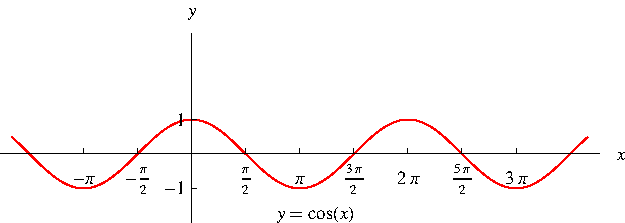
\includegraphics[width=12cm]{inverse-trig/pictures/07-06-arccosa.pdf}%
%}%
%\only<2>{%
%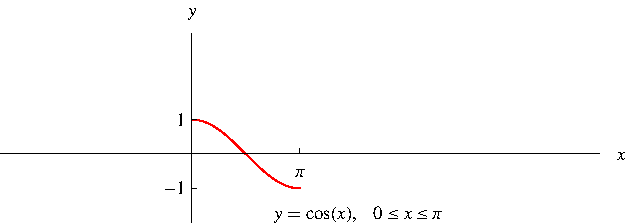
\includegraphics[width=12cm]{inverse-trig/pictures/07-06-arccosb.pdf}%
%}%
%\only<handout:0| 3->{%
%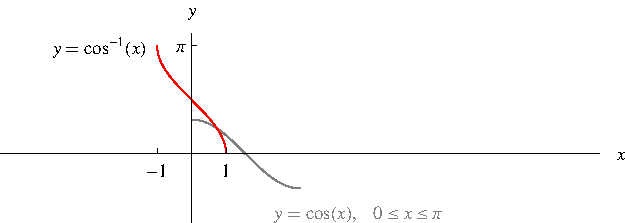
\includegraphics[width=12cm]{inverse-trig/pictures/07-06-arccosc.pdf}%
%}%
\psset{xunit=0.6cm,yunit=0.6cm}
\begin{pspicture}(-5,-1.4)(10,1.4)
\tiny
\psaxes[labels=none, ticks=x, Dx=1.570796327, Dy=1] {<->}(0,0)(-4,-1.4)(10,3.4)
\psLabels{10}{3.4}
\uncover<1>{\psplot[linecolor=red, plotpoints=1000]{-4}{10}{x 57.295779513 mul cos}
\rput[t](3.5, 1){$y=\cos x$}
}
\uncover<2>{\psplot[linecolor=red, plotpoints=1000]{0}{3.141592654}{x 57.295779513 mul cos}
\rput[t](3.5, 1){$y=\cos x, \quad 0\leq x\leq \pi$}
}
\uncover<3->{\psplot[linecolor=gray, plotpoints=1000]{0}{3.141592654}{x 57.295779513 mul cos}
\rput[t](3.5, 1){\color{gray}$y=\cos x, \quad 0\leq x\leq \pi$}

\psplot[linecolor=red, plotpoints=1000]{-1}{1}{x ACOS}
\psline(-0.1,3.141592654)(0.1,3.141592654)
\rput[l](0.15,3.141592654){$\pi$}
\psline(-1,-0.1)(-1,0.1)
\rput[t](-1,-0.1){$-1$}
\psline(1,-0.1)(1,0.1)
\rput[t](1,-0.1){$1$}
\rput[r](-0.6, 0.4){$y=\Arccos x$}
}

\rput[t](-3.14, -0.3){$-\pi$}
\rput[t](-1.57, -0.3){$-\frac{\pi}{2}$}
\rput[t](1.57, -0.3){$\frac{\pi}{2}$}
\rput[t](3.14, -0.3){$\pi$}
\rput[t](4.71, -0.3){$\frac{3\pi}{2}$}
\rput[t](6.28, -0.3){$2\pi$}
\rput[t](7.85, -0.3){$\frac{5\pi}{2}$}
\rput[t](9.42, -0.3){$3\pi$}
\rput[br](-0.2,1){\tiny $1$}

\end{pspicture}

\begin{columns}[c]
\column{.65\textwidth}
\begin{itemize}
\item<1->  Same for $\cos x$.
\item<2->  Restrict the domain to $[0, \pi ]$.
\item<3->  The inverse is called $\arccos$ or $\cos^{-1}$.
\item<5->  $\Arccos (x) = y \Leftrightarrow \cos y = x$ and $0 \leq y \leq \pi$.
\end{itemize}
\column{.35\textwidth}
\uncover<4->{%
%\uncover<4->{%
%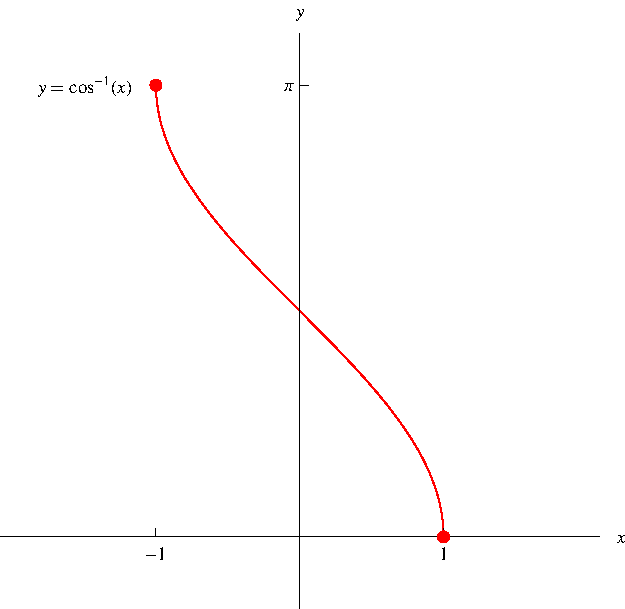
\includegraphics[height=4cm]{inverse-trig/pictures/07-06-arccosd.pdf}%
%}%
\psset{xunit=1.2cm,yunit=1.2cm}
\begin{pspicture}(-5,-1.4)(10,1.4)
\tiny
\psaxes[labels=none, ticks=none] {<->}(0,0)(-2,-0.5)(1.6,3.7)
\psLabels{1.6}{3.7}
\psplot[linecolor=red, plotpoints=1000]{-1}{1}{x ACOS}
\psline(-0.1,3.141592654)(0.1,3.141592654)
\rput[l](0.15,3.141592654){$\pi$}
\psline(-1,-0.1)(-1,0.1)
\rput[t](-1,-0.1){$-1$}
\psline(1,-0.1)(1,0.1)
\rput[t](1,-0.1){$1$}
\rput[r](-0.6, 2){$y=\Arccos x$}
\end{pspicture}
}%
\end{columns}
\end{frame}
% end module arccos-def


\end{document}
